%%%%%%%%%% *** The Title %%%%%%%%%%
\title[]{허리케인\\\small{제11장}}

\begin{frame}[plain] %title page
	\titlepage
\end{frame}


\section{허리케인의 개요}

\begin{frame}[t]{허리케인}
	\begin{tabular}{ll}
		\begin{minipage}[t]{0.6\textwidth}\scriptsize
			\begin{figure}[t]
				\includegraphics[trim=30 30 230 540, clip, 
				page=331, width=\textwidth]{\bookfile}
			\end{figure}
		\end{minipage}	
		&
		\begin{minipage}[t]{0.35\textwidth} \scriptsize	
			\begin{itemize}
				\item 열대 및 아열대 해안 주위에 형성.
				\item 열대성 폭풍의 이름은 지역마다 다르다
				\item 태풍(태평양 북서부), 
				사이클론(태평양 남서부 및 인도양), 
				윌리윌리(오세아니아), 
				허리케인(북아메리카)				
			\end{itemize}			
		\end{minipage}
	\end{tabular}
\end{frame}


\begin{frame}[t]{허리케인 프랜}
	\begin{tabular}{ll}
		\begin{minipage}[t]{0.6\textwidth}\scriptsize
			\begin{figure}[t]
				\includegraphics[trim=50 440 220 50, clip, 
				page=332, width=\textwidth]{\bookfile}
			\end{figure}
		\end{minipage}	
		&
		\begin{minipage}[t]{0.35\textwidth} \scriptsize	
			

		\end{minipage}
	\end{tabular}
\end{frame}


\begin{frame}[t]{허리케인}
	\begin{tabular}{ll}
		\begin{minipage}[t]{0.5\textwidth}\scriptsize
			\begin{figure}[t]
				\includegraphics[trim=280 320 50 120, clip, 
				page=331, width=\textwidth]{\bookfile}
			\end{figure}
		\end{minipage}	
		&
		\begin{minipage}[t]{0.45\textwidth} \scriptsize	

			\begin{itemize}
				\item 강한 저기압 중심(강한 수렴과 저기압성 회전)을 가지고 있으며, 
				\item 강한 뇌우 및 120 km/h(약 34 m/s)를 넘는 풍속을 가짐.
				\item 지름이 100~1500k m 정도.(평균 600km)
				\item 강한 기압경도를 가져 풍속이 빠름.
				\item 중심 기압이 950 hPa까지 내려갈 수 있음
			\end{itemize}

		\end{minipage}
	\end{tabular}
\end{frame}


\begin{frame}[t]{허리케인의 구조}
	\begin{tabular}{ll}
		\begin{minipage}[t]{0.3\textwidth}\scriptsize
			\begin{figure}[t]
				\includegraphics[trim=420 360 70 90, clip, page=333, width=0.8\textwidth]{\bookfile}
			\end{figure}
		\end{minipage}	
		&
		\begin{minipage}[t]{0.65\textwidth} \scriptsize	
			
			\begin{itemize}
				\item 각운동량 보존은 허리케인 중심에서 강한 풍속을 설명
				\item 120 $\rm{km/h}$의 풍속은 허리케인 중심에 해당하며, 외곽지역의 바람은 그 보다 풍속이 느리다. 
				\item 허리케인의 중심에서 500 $\rm{km}$ 떨어진 지점에서 5 $\rm{km/h}$의 속력을 가진 공기 덩이가 출발할 경우, 마찰을 무시하면 반경 10 km 근처에서는 250 $\rm{km/h}$의 속력을 가짐.
				\item 스케이터의 팔이 축 주위로 원운동하는데, 팔을 안으로 당기면 원운동 반경이 줄어들어 팔은 더 빨라지고 몸이 따라가서 회전속도 증가.
			\end{itemize}

		\end{minipage}
	\end{tabular}
\end{frame}



\begin{frame}[t]{허리케인 형성}
	\begin{tabular}{ll}
		\begin{minipage}[t]{0.6\textwidth}\scriptsize
			\begin{figure}[t]
				\includegraphics[trim=30 30 230 540, clip, page=331, width=\textwidth]{\bookfile}
			\end{figure}
		\end{minipage}	
		&
		\begin{minipage}[t]{0.35\textwidth} \scriptsize	
			\questionset{적도에서 열대성 저기압이 잘 발달하지 않는 이유를 배경회전을 고려하여 설명하시오.}
			\solutionset{
			왼쪽 그림과 같이 배경회전이 없는 경우 각운동량 보존을 사용하면 중심으로부터 $r2$만큼 떨어진 곳으로 이동했을 때 지면에 대한 상대속도 $v2$를 쉽게 구할 수 있다. 
			그러나 배경회전이 있으면 지면에 대한 상대적 각운동량 및 배경회전에 의한 각운동량을 고려해야 한다. r1에서 지면에 대해 v1의 상대 속도로 움직이는 공기를 생각하자. 
			이 공기는 지면 자체가 돌고 있기 때문에 $ωr1^2$이라는 배경회전 각운동량도 동시에 가지고 있다. 이러한 배경 회전 각운동량을 고려하면 r2으로 회전반지름이 바뀔 때 매우 큰 v2’라는 값으로 바뀐다. 
			이와 같이 배경회전이 있으면 매우 큰 회전속도를 갖게 된다.}
		\end{minipage}
	\end{tabular}
\end{frame}


\begin{frame}[t]{허리케인의 구조}
	\begin{tabular}{ll}
		\begin{minipage}[t]{0.6\textwidth}\scriptsize
			\begin{figure}[t]
				\includegraphics[trim=305 230 0 330, clip, 
				page=332, width=\textwidth]{\bookfile}
			\end{figure}
		\end{minipage}	
		&
		\begin{minipage}[t]{0.35\textwidth} \scriptsize	

			\begin{itemize}
				\item 저기압의 중심에서 수렴하여 상승(적란운 생성) 후, 상층에서 발산
				\item 허리케인의 눈에서 기압은 제일 낮고, 풍속도 느림.
				\item 눈벽: 폭풍의 중심을 둘러싼 도넛 모양의 벽  \\
				 최대 풍속, 가장 강한 강우
				\item 강우선 : 점점 약해지는 곡선 이룬 구름층 \\
				강우선이 눈벽을 둘러쌈
			\end{itemize}
			
		\end{minipage}
	\end{tabular}
\end{frame}



\begin{frame}[t]{허리케인의 구조}
	\begin{tabular}{ll}
		\begin{minipage}[t]{0.45\textwidth}\scriptsize
			\begin{figure}[t]
				\includegraphics[trim=305 230 0 330, clip, 
				page=332, width=\textwidth]{\bookfile}
			\end{figure}
		\end{minipage}	
		&
		\begin{minipage}[t]{0.5\textwidth} \scriptsize	

			\begin{itemize}
				\item 허리케인의 상부에서 유출되는 공기는 지표면에서 유입되는 공기가 쌓이는 것을 막아 저기압을 유지하는데 중요한 역할을 함
				\item 눈에서 침강하는 공기는 압축에 의해 온도 상승
				\item 눈벽은 바람과 강수가 가장 강한 지역
				\item 안쪽을 휘감는 고온 다습한 수증기는 허리케인 중심 주변에 바퀴모양의 강수대를 형성 
			\end{itemize}
			
		\end{minipage}
	\end{tabular}
\end{frame}



\begin{frame}[t]{허리케인의 구조}
	\begin{tabular}{ll}
		\begin{minipage}[t]{0.6\textwidth}\scriptsize
			\begin{figure}[t]
				\includegraphics[trim=40 30 350 440, clip, 
				page=333, width=\textwidth]{\bookfile}
			\end{figure}
		\end{minipage}	
		&
		\begin{minipage}[t]{0.35\textwidth} \scriptsize	
			\begin{itemize}
				\item 태풍의 하층에서는 사이클론(반시계 방향) 순환을 형성하여 중심을 향해 불어 들어 가는 반면, 상층에서는 반사이클론(시계방향) 순환을 형성하여 밖으로 불어 나감.
				\item  풍속의 최대 지역은 태풍 중심 부근인 눈벽이며, 중심을 둘러싼 도넛 모양의 벽을 의미한다. 
				이 위치 에서 기압 경도력이 최대가 된다.
			\end{itemize}

		\end{minipage}
	\end{tabular}
\end{frame}


\section{허리케인의 생성과 소멸}

\begin{frame}[t]{허리케인의 생성 시기 및 위치}
	\begin{tabular}{ll}
		\begin{minipage}[t]{0.475\textwidth}\scriptsize
			\begin{figure}[t]
				\includegraphics[trim=50 50 330 500, clip, 
				page=334, width=\textwidth]{\bookfile}
			\end{figure}
		\end{minipage}	
		&
		\begin{minipage}[t]{0.475\textwidth} \scriptsize	
			\begin{figure}[t]
				\includegraphics[trim=350 440 30 120, clip, 
				page=334, width=\textwidth]{\bookfile}
			\end{figure}

		\end{minipage}
	\end{tabular}
	\begin{itemize}
		\scriptsize	
		\item 늦여름과 초가을에 자주 발생 (바닷물 온도가 $\rm{27^{\circ}C}$ 이상, 열과 수증기 제공)
		\item 위도 $30^{\circ}$ 이상에서는 생성x (바닷물 온도조건 충족 x 때문)
		\item 적도로부터 $5^{\circ}$이내에서는 생성x (전향력이 너무 약하여 회전 운동 발생x)
	\end{itemize}
\end{frame}



\begin{frame}[t]{허리케인의 형성}
	\begin{tabular}{ll}
		\begin{minipage}[t]{0.9\textwidth}\scriptsize
			\begin{figure}[t]
				\includegraphics[trim=30 490 30 50, clip, 
				page=335, width=\textwidth]{\bookfile}
			\end{figure}
		\end{minipage}	
		&
		\begin{minipage}[t]{0.05\textwidth} \scriptsize	

		\end{minipage}
	\end{tabular}
	\begin{itemize} \scriptsize	
		\item 열대 요란(불안정한 구름, 뇌우)이 생성
		\item 편동풍 파동에 의해 점진적으로 동쪽에서 서쪽으로 이동
		\item 열대 요란으로부터 형성되는 뇌우에서 잠열이 방출, 요란 내부의 기온이 상승, 밀도가 낮아지게 되고, 지표 기압 감소, 저기압성 순환 발달, 수평기압경도 증가, 지상풍속 증가, 추가 수증기 공급, 폭풍 성장.
	\end{itemize}
\end{frame}


\begin{frame}[t]{허리케인의 형성}
	\begin{tabular}{ll}
		\begin{minipage}[t]{0.475\textwidth}\scriptsize
			\begin{itemize}
				\item 발달 중인 열대성 저기압 상부에서는 대기가 바깥쪽으로 흐르는 데, 만약 이 바람이 없으면 지표면의 압력이 상승되어 추가적 폭풍 발달이 저해됨.
				\item 많은 열대 요란이 발생하지만, 지속적으로 강력한 폭우를 만들지 않으면 90 \%의 열대요란은 소멸.
				\item 이러한 상황에서 상층에서 고기압이 발달하여 발산이 일어나면 풍속에 따라 열대성 저기압($ \sim~63~\rm{km/h}$), 열대성 폭풍($\sim~119~\rm{km/h}$), 
				허리케인($119~{km/h}\sim$)으로 성장.
				\item 낮은 비율의 열대요란이 열대성 저기압으로 진화하지만 큰 규모의 열대성 저기압은 열대성 폭풍이 되고, 훨씬 큰 규모의 열대성 폭풍은 허리케인으로 강화.
			\end{itemize}
		\end{minipage}	
		&
		\begin{minipage}[t]{0.475\textwidth} \scriptsize
			\questionset{적도 근처에서 형성되는 열대성 폭풍은 고위도의 저기압처럼 회전운동을 하지 않는 이유는 무엇인지 설명하시오.}
			\solutionset{적도 근처는 코리올리 힘이 매우 작기 때문에 고위도의 저기압과 같은 회전운동을 하지 않는다. 대신 편동풍 파동에 의해서 저기압성 회전이 발달할 수 있다. \newline}	
			
			\questionset{열대성 폭풍과 열대성 저기압 중 풍속이 강한 것은 무엇인가?}
			\solutionset{열대성 저기압은 풍속이 $63~\rm{km/h}$보다 느린 경우를, 열대성 폭풍은 $63~\rm{km/h}$보다 빠르고 $119~\rm{km/h}$ 보다는 느린 경우를 말한다.
			우리나라에서는 열대성 폭풍 이상을 보통 태풍이라고 부른다. 미국에서는 $119~\rm{km/h}$ 이상의 풍속을 가진 경우 허리케인이라고 부른다.\newline}

		\end{minipage}
	\end{tabular}
\end{frame}


\begin{frame}[t]{허리케인의 소멸}
	\begin{tabular}{ll}
		\begin{minipage}[t]{0.475\textwidth}\scriptsize
			\begin{itemize}
				\item 잠열이 차단되면 소멸됨
				\item 허리케인이 차가운 물이나 육지로 이동하는 경우
				\item 상층의 큰 규모의 흐름이 허리케인의 성장에 유리하지 않을 때
			\end{itemize}

			\questionset{허리케인은 어떻게 소멸하는가?}
			\solutionset{허리케인의 에너지원인 수증기 공급이 줄어들면 세력이 약화된다. \\
					- 육지로 이동하는 경우\\
					- 찬 해수 지역으로 이동하는 경우\\
					- 해수의 온도는 높으나 온도가 높은 층의 깊이가 얕은 경우 \newline}
			
		\end{minipage}	
		&
		\begin{minipage}[t]{0.475\textwidth} \scriptsize	
			
			\questionset{허리케인의 강도는 육지로 이동할 때 왜 빠르게 약화되는지 설명하시오.}
			\solutionset{허리케인이 육지로 이동하게 되면 따뜻함과 수증기의 공급원이 차단된다. 일반적인 경우 육지가 바다보다 더 빨리 냉각이 일어나게 되어 하층 공기가 가열되기 보다 냉각된다. 뿐만 아니라 마찰이 증가하여 표층 풍속이 급속히 감소하게 되고, 저기압 중심으로 바람이 보다 직접적으로 들어가게 되어 기압차가 감소하게 되어 약화된다.}

			\questionset{열대 요란의 강화를 방해하는 두 가지 요소를 쓰시오.}
			\solutionset{ - 무역풍 역전: 아열대고기압의 영향을 받은 지역에서 나타나는 침강으로 인하여 형성된 강한 역전은 대기의 상승력을 감소시키고 뇌우의 발생을 억제
					- 강한 상층 바람: 상층의 강한 바람은 구름 상부에서 발산된 잠열을 소산되게 하여 열대 요란의 지속적인 성장과 발달을 방해}
			
		\end{minipage}
	\end{tabular}
\end{frame}



\begin{frame}[t]{허리케인의 명칭}
	\begin{tabular}{ll}
		\begin{minipage}[t]{0.5\textwidth}\scriptsize
			\begin{figure}[t]
				\includegraphics[trim=250 120 30 175, clip, 
				page=336, width=0.9\textwidth]{\bookfile}
			\end{figure}
		\end{minipage}	
		&
		\begin{minipage}[t]{0.45\textwidth} \scriptsize	
			\questionset{과거 열대성 저기압의 이름은 어떻게 명명하였는가?}
			\solutionset{싫어하는 정치인의 이름, 여성의 이름 등}
			
		\end{minipage}
	\end{tabular}
\end{frame}


\begin{frame}[t]{태풍}
	\begin{tabular}{ll}
		\begin{minipage}[t]{0.475\textwidth}\scriptsize
			\begin{itemize}
				\item 생성장소: 위도 $5\rm^{\circ}~\sim~20\rm^{\circ}$ 사이의 열대 및 아열대 해상
				\item 해수면의 온도가 $27~\rm{^{\circ}C}$ 보다 높은 곳
				열과 수증기를 공급 
				\item 생성시기: 늦여름~초가을(수온이 이때가 절정)
				\item 원동력: 수증기의 응결로 인해 방출되는 잠열
				\item 잠열이 방출되면 공기덩이가 주변보다 가벼워지고 추가로 상승할 수 있음
				
			\end{itemize}
		\end{minipage}	
		&
		\begin{minipage}[t]{0.475\textwidth} \scriptsize	
			\questionset{태풍의 이름은 모두 몇개인가?}
			\solutionset{14개 나라 각 10개씩 140개를 5개 조로 나눈다.\newline}

			\questionset{태풍의 이름은 어떻게 퇴출되는가?}
			\solutionset{심각한 피해를 입힌 태풍의 경우 회원국이 요청을하면 영구 제외되고 새로운 이름으로 교체된다.}
			
		\end{minipage}
	\end{tabular}
\end{frame}




\section{허리케인의 피해}

\begin{frame}[t]{허리케인의 피해}
	\begin{tabular}{ll}
		\begin{minipage}[t]{0.475\textwidth}\scriptsize
			\begin{figure}[t]
				\includegraphics[trim=350 30 50 480, clip, 
				page=337, width=\textwidth]{\bookfile}
			\end{figure}
		\end{minipage}	
		&
		\begin{minipage}[t]{0.475\textwidth} \scriptsize	
			\begin{figure}[t]
				\includegraphics[trim=350 480 40 50, clip, 
				page=338, width=\textwidth]{\bookfile}
			\end{figure}			
		\end{minipage}
	\end{tabular}
	\begin{itemize}
		\item 허리케인의 파괴적 영향은 생성된 곳과 다른 곳에서 나타남
	\end{itemize}			
\end{frame}

\begin{frame}[t]{허리케인의 피해}
	\begin{tabular}{ll}
		\begin{minipage}[t]{0.5\textwidth}\scriptsize
			
		\end{minipage}	
		&
		\begin{minipage}[t]{0.45\textwidth} \scriptsize	
			\begin{itemize}
				\item 많은 인명 피해가 나타날 수 있음.
				\item 
				\item 
			\end{itemize}

		\end{minipage}
	\end{tabular}
\end{frame}


\begin{frame}[t]{사피어-심프슨 허리케인 등급}
	\begin{tabular}{ll}
		\begin{minipage}[t]{0.4\textwidth}\scriptsize
			\begin{figure}[t]
				\includegraphics[trim=50 530 350 100, clip, 
				page=338, width=\textwidth]{\bookfile}
			\end{figure}
		\end{minipage}	
		&
		\begin{minipage}[t]{0.55\textwidth} \scriptsize	
			\begin{figure}[t]
				\includegraphics[trim=350 30 50 585, clip, 
				page=338, width=0.8\textwidth]{\bookfile}
			\end{figure}
			\begin{itemize}
				\item 기압, 풍속, 폭풍해일에 기반하여 $1~\sim~5$등급으로 강도를 구별
			\end{itemize}
			\questionset{Saffir-Simpson 등급의 목적은 무엇인가?}
			\solutionset{허리케인의 강도를 예측하여 이로 인하여 예상될 수 있는 피해를 예측하기 위해서이다. 이는 허리케인의 잠재적 피해 정도를 예측하여 시설을 점검하고 적절한 예방 조치를 취할 수 있도록 도움을 준다.}

		\end{minipage}
	\end{tabular}
\end{frame}

\begin{frame}[t]{폭풍 해일}
	\begin{tabular}{ll}
		\begin{minipage}[t]{0.5\textwidth}\scriptsize
			\begin{figure}[t]
				\includegraphics[trim=0 0 300 540, clip, 
				page=339, width=\textwidth]{\bookfile}
			\end{figure}
			
			\begin{itemize}\scriptsize
				\item 65~80 km 정도의 범위로 태풍의 눈이 상륙하는 지점 근처 해안에 영향을 줌
				\item 표면에 부는 강한 해풍에 의해 바닷물의 수위가 상승	
			\end{itemize}
		\end{minipage}	
		&
		\begin{minipage}[t]{0.45\textwidth} \scriptsize	
			\begin{figure}[t]
				\includegraphics[trim=330 400 50 55, clip, 
				page=339, width=\textwidth]{\bookfile}
			\end{figure}
		\end{minipage}
	\end{tabular}
\end{frame}


\begin{frame}[t]{허리케인 Sandy에 의한 피해}
	\begin{tabular}{ll}
		\begin{minipage}[t]{0.475\textwidth}\scriptsize
			\begin{figure}[t]
				\includegraphics[trim=30 30 310 480, clip, 
				page=340, width=0.9\textwidth]{\bookfile}
			\end{figure}
		\end{minipage}	
		&
		\begin{minipage}[t]{0.475\textwidth}\scriptsize	
			\begin{figure}[t]
				\includegraphics[trim=350 320 30 120, clip, 
				page=340, width=0.9\textwidth]{\bookfile}
			\end{figure}

		\end{minipage}
	\end{tabular}
\end{frame}


\begin{frame}[t]{상승하는 해수위의 위험}
	\begin{tabular}{ll}
		\begin{minipage}[t]{0.5\textwidth}\scriptsize
			\begin{figure}[t]
				\includegraphics[trim=30 500 350 50, clip, 
				page=341, width=\textwidth]{\bookfile}
			\end{figure}
		\end{minipage}	
		&
		\begin{minipage}[t]{0.45\textwidth} \scriptsize	
			\questionset{지구 온난화에 기인한 해수위 상승은 해안 저지대에 어떤 위험을 초래하는가?}
			\solutionset{지구온난화의 반응으로 해수위가 상승하면서저디대 삼국주 지대는 풍풍 해일에 훨씬 더 취약하게 될 것이다. 
			또한 조석 주기와 폭풍 해일이 더해지는 경우 그 피해는 매우 심각해 질 수 있다. }

		\end{minipage}
	\end{tabular}
\end{frame}


\begin{frame}[t]{허리케인의 피해}
	\begin{tabular}{ll}
		\begin{minipage}[t]{0.4\textwidth}\scriptsize
			\begin{figure}[t]
				\includegraphics[trim=30 30 230 540, clip, page=331, width=\textwidth]{\bookfile}
			\end{figure}
		\end{minipage}	
		&
		\begin{minipage}[t]{0.55\textwidth} \scriptsize	
			\questionset{허리케인의 피해는 세 가지 범주로 나눌 수 있다. 각 범주를 설명하고 가장 큰 사망자를 내는 것은 무엇인지 쓰시오.}
			\solutionset{해안 지역 피해의 대부분과 허리케인으로 인한 사망의 90 \%가 폭풍 해일 때문이다. 
			폭풍 해일은 저기압으로 인한 해풍으로 인해 수위가 높아지고, 만조가 나타나거나 만이나 강의 어귀인 경우 피해가 심각할 수 있다. 특히 인구 밀집 지대가 보통 해안지대이므로 해발 고도가 낮은 연안 지역의 피해가 심각할 수 있다. 방글라데시의 삼각주 지역은 대부분의 육지가 해발 2m 미만이므로 이러한 지역에서 사이클론이 나타날 경우 20만명 이상의 사망자가 나타날 수 있다.
			하지만 더 넓은 지역에 영향을 미치는 것은 강풍이다. \\
			강풍으로 적어도 2백만 명이 살 집을 잃었고, 백만명 이상이 이주했다.\\
			허리케인에 의한 또하나의 피해는 폭우이다.}
		\end{minipage}
	\end{tabular}
\end{frame}


\begin{frame}[t]{위험 반원과 안전 반원}
	\begin{tabular}{ll}
		\begin{minipage}[t]{0.55\textwidth}\scriptsize
			\begin{figure}[t]
				\includegraphics[trim=30 30 350 490, clip, 
				page=341, width=\textwidth]{\bookfile}
			\end{figure}
		\end{minipage}	
		&
		\begin{minipage}[t]{0.4\textwidth} \scriptsize	
			\begin{itemize}
				\item 안전반원/가항반원	(navigable semicircle) : 풍속이 
				상대적으로 느리다.
				\item 위험반원 (dangerous semicircle): 풍속이 
				상대적으로 빠르다.
			\end{itemize}

		\end{minipage}
	\end{tabular}
\end{frame}





\section{허리케인의 강도 추정}


\begin{frame}[t]{드롭 존데}
	\begin{tabular}{ll}
		\begin{minipage}[t]{0.4\textwidth}\scriptsize
			\begin{figure}[t]
				\includegraphics[trim=350 30 50 360, clip, 
				page=342, width=0.9\textwidth]{\bookfile}
			\end{figure}
		\end{minipage}	
		&
		\begin{minipage}[t]{0.55\textwidth} \scriptsize	
			\begin{itemize}
				\item 허리케인의 강도 추정을 위해서는 정확한 관측이 필요함.
				\item 상층 바람이 지상 바람보다 빠름은 알고 있었음.
				\item 1997년, GPS를 갖춘 drop windsonde(드롭 존데)가 개발되어, 허리케인 내부의 기압, 습도, 풍속, 풍향을 정밀 측정 
    			\item 직경: $7~\rm{cm}$, 길이: $40~\rm{cm}$, 무게: $0.4~\rm{kg}$
			\end{itemize}
			
			바람 측정 : 비접촉식표면조도계(scatterometer) 활용
		\end{minipage}
	\end{tabular}
\end{frame}


\begin{frame}[t]{위성자료 활용}
	\begin{tabular}{ll}
		\begin{minipage}[t]{0.475\textwidth}\scriptsize
			\begin{figure}[t]
				\includegraphics[trim=320 30 50 540, clip, 
				page=343, width=\textwidth]{\bookfile}
			\end{figure}
		\end{minipage}	
		&
		\begin{minipage}[t]{0.475\textwidth} \scriptsize	
			\begin{itemize}
				\item 
			   
			\end{itemize}

		\end{minipage}
	\end{tabular}
\end{frame}


\begin{frame}[t]{위성자료 활용}
	\begin{tabular}{ll}
		\begin{minipage}[t]{0.475\textwidth}\scriptsize
			\begin{figure}[t]
				\includegraphics[trim=320 440 30 30, clip, 
				page=344, width=\textwidth]{\bookfile}
			\end{figure}
		\end{minipage}	
		&
		\begin{minipage}[t]{0.475\textwidth} \scriptsize	
			\begin{itemize}
				\item 강우량과 운고 측정
				\item 다른 부분의 강우량 패턴을 보는것.
				\item 열대성 강우량 측정 위성(Tropical Rainfall Measuring Mission, TRMM)
				\item 열탑(hot towers) : 거대한 적란운의 하나
			   
			\end{itemize}

		\end{minipage}
	\end{tabular}
\end{frame}






\section{허리케인 탐지와 진로 분석}

\begin{frame}[t]{인공위성}
	\begin{tabular}{ll}
		\begin{minipage}[t]{0.6\textwidth}\scriptsize
			\begin{figure}[t]
				\includegraphics[trim=30 420 250 50, 
				clip, page=345, width=\textwidth]{\bookfile}
			\end{figure}
		\end{minipage}	
		&
		\begin{minipage}[t]{0.35\textwidth} \scriptsize	
			\begin{itemize}
				\item 허리케인의 탐지 및 이동 경로 파악에 큰 도움을 줌
				\item 원격 관측이 가능하지만, 풍속을 정확히 측정할 수 없는 단점
			\end{itemize}
			
		\end{minipage}
	\end{tabular}
\end{frame}


\begin{frame}[t]{항공기}
	\begin{tabular}{ll}
		\begin{minipage}[t]{0.5\textwidth}\scriptsize
			\begin{figure}[t]
				\includegraphics[trim=30 465 295 50, clip, 
				page=346, width=\textwidth]{\bookfile}
			\end{figure}
		\end{minipage}	
		&
		\begin{minipage}[t]{0.45\textwidth} \scriptsize	
			\begin{itemize}
				\item 미국은 관측을 위한 항공기가 많으나, 우리나라는 거의 없다.
				\item 관측장비를 장착한 항공기를 이용하여 허리케인을 통과하거나 주변을 통과하며 관측
				\item 육지와 근거리에서만 관측 가능
				\item Snapshot data(일부의 자료)를 제공(하지만 긴요하게 쓰임)
				\item 허리케인의 구조와 특징을 이해하는 데 큰 도움을 제공
			\end{itemize}

		\end{minipage}
	\end{tabular}
\end{frame}




\begin{frame}[t]{레이더}
	\begin{tabular}{ll}
		\begin{minipage}[t]{0.45\textwidth}\scriptsize
			\begin{figure}[t]
				\includegraphics[trim=30 370 290 50, clip, 
				page=347, width=0.8\textwidth]{\bookfile}
			\end{figure}
			
			레이더: 320km 범위내에서 감지 가능, 도플러 기상 레이더로 강수 모니터링 풍향과 풍속, 강수량 측정 가능
		\end{minipage}	
		&
		\begin{minipage}[t]{0.45\textwidth} \scriptsize	
			\begin{figure}[t]
				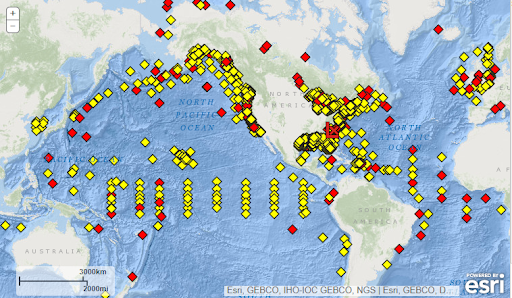
\includegraphics[width=0.8\textwidth]{./images/buye.png}
			\end{figure}
			
			해상 부이: 해상에서 원격으로 허리케인 정보 제공(멕시코만, 대서양 연안)

		\end{minipage}
	\end{tabular}
\end{frame}




\begin{frame}[t]{허리케인의 피해}
	\begin{tabular}{ll}
		\begin{minipage}[t]{0.95\textwidth}\scriptsize
			\begin{figure}[t]
				\includegraphics[trim=0 0 0 510, clip, 
				page=345, width=\textwidth]{\bookfile}
			\end{figure}
		\end{minipage}	
		&
		\begin{minipage}[t]{0.01\textwidth} \scriptsize	
			
		\end{minipage}
	\end{tabular}
\end{frame}



\begin{frame}[t]{볼트락}
	\begin{tabular}{ll}
		\begin{minipage}[t]{0.5\textwidth}\scriptsize
			\begin{figure}[t]
				\includegraphics[trim=330 50 50 460, clip, 
				page=347, width=\textwidth]{\bookfile}
			\end{figure}
		\end{minipage}	
		&
		\begin{minipage}[t]{0.45\textwidth} \scriptsize	
			\questionset{허리케인을 추적하고 기상 예보의 발달을 가져온 4가지 기기를 쓰고, 설명하시오.}
			\solutionset{
					인공위성: 넓은 범위에 대한 원격 관측이 가능하고, 허리케인의 발생이나 이동경로 추적에 용이함.\\
					항공기: 비행 거리 제한으로 인해 허리케인이 근접했을 때 관측이 가능하지만, 직접 여러가지 정보를 관측하여 태풍의 구조와 특성 이해에 큰 도움을 제공해 줌.\\
					레이더: 도플러 효과를 이용하여 풍향, 풍속, 강수량을 측정할 수 있음.\\
					해상 부이: 해양의 고정된 위치에서 육지로 다가오는 허리케인의 풍향, 풍속, 기압 등의 실제 정보를 제공하며, 육지에서 먼 곳에서 관측 정보를 제공한다는 점이 장점임. }

		\end{minipage}
	\end{tabular}
\end{frame}




\begin{frame}[t]{수퍼 태풍 하이난}
	\begin{tabular}{ll}
		\begin{minipage}[t]{0.475\textwidth}\scriptsize
			\begin{figure}[t]
				\includegraphics[trim=350 410 30 110, clip, 
				page=348, width=\textwidth]{\bookfile}
			\end{figure}
		\end{minipage}	
		&
		\begin{minipage}[t]{0.475\textwidth} \scriptsize	
			\begin{figure}[t]
				\includegraphics[trim=350 50 30 370, clip, 
				page=348, width=\textwidth]{\bookfile}
			\end{figure}

		\end{minipage}
	\end{tabular}
\end{frame}




\begin{frame}[t]{허리케인 예보}
	\begin{tabular}{ll}
		\begin{minipage}[t]{0.6\textwidth}\scriptsize
			\begin{figure}[t]
				\includegraphics[trim=250 410 50 50, clip, 
				page=349, width=\textwidth]{\bookfile}
			\end{figure}
		\end{minipage}	
		&
		\begin{minipage}[t]{0.35\textwidth} \scriptsize	
			\begin{itemize}
				\item 허리케인 예보: 경로 예보
				
				\item 허리케인 주의보: 풍속이 열대 폭풍 수준에 도달할 것으로 보이면 48시간 전에 발령
				\item 허리케인 경보: 열대 폭풍이 지나갈 것으로 예상되면 36시간 전에 발령
				
			\end{itemize}

		\end{minipage}
	\end{tabular}
\end{frame}

